% Append after the manuscript's existing appendices.
% Do not issue another \appendix if appendix mode is already active.

\section{Derivation of the PL gradient-root updates}
\label{app:gotham_pl_updates}

Fix an outer iteration $k$ and abbreviate
$\Phi=\hat\Phi^{(k)}$, $\hat\theta=\hat\theta^{(k)}$.
All regressors, auxiliary operators, and inverse parameters below are
held fixed during this homotopy construction. The regressor is rebuilt
only after the outer update. The local map and residual are
\begin{align}
\label{eq:WS_pseudolinear_operator_k}
    \mathcal W_{\mathrm{PL}}^{(k)}(\theta)&=\Phi\theta,\\
\label{eq:WS_PL_residual_k}
    r_{\mathrm{PL}}^{(k)}(\theta)&=C-\Phi\theta.
\end{align}
For the loss~\eqref{eq:WS_loss_k}, define
\begin{equation}
\label{eq:WS_gradient_hessian_definitions}
    G=\Phi^\top\Phi,\qquad b=\Phi^\top C,\qquad
    g=G\hat\theta-b.
\end{equation}

\subsection{Residual coefficients and deformation terms}

The gradient-root operator and its derivatives satisfy
\begin{align}
\label{eq:gradient_root_operator}
    \mathcal N_{G,\mathrm{PL}}^{(k)}(\theta)&=G\theta-b,\\
\label{eq:gradient_root_derivatives}
    D\mathcal N_{G,\mathrm{PL}}^{(k)}(\theta)[h]&=Gh,
    \qquad D^p\mathcal N_{G,\mathrm{PL}}^{(k)}=0\quad(p\ge2).
\end{align}
Substitution of $\phi(q)=\hat\theta+\sum_{m\ge1}\theta_mq^m$
therefore gives
\begin{equation}
\label{eq:gradient_root_residuals}
    R_1=g,\qquad R_m=G\theta_{m-1}\quad(m\ge2).
\end{equation}
With $H=I$, $\hbar=-\eta$, and a fixed linear
$P=\mathcal L^\dagger$, the HODE recursion becomes
\begin{align}
\label{eq:gradient_root_theta1_general}
    \theta_1&=-\eta Pg,\\
\label{eq:gradient_root_thetam_general}
    \theta_m&=(I-\eta PG)\theta_{m-1},\qquad m\ge2.
\end{align}
Hence, setting $B=I-\eta PG$,
\begin{equation}
\label{eq:PL_gradient_arbitrary_order}
    \theta_m=-\eta B^{m-1}Pg,\qquad
    \Delta_M=-\eta\sum_{j=0}^{M-1}B^jPg.
\end{equation}
For this fixed quadratic loss, the same increment is obtained by $M$
successive preconditioned gradient steps with unchanged $\Phi$, $P$,
and $\eta$. Indeed, the increments of
$x_j=x_{j-1}-\eta P(Gx_{j-1}-b)$, $x_0=\hat\theta$, obey the same
recursion as $\theta_j$. This equivalence concerns the inner steps;
reconstructing the latent signals between those steps changes the problem.

\subsection{Classical first-order special cases}

For $M=1$,
\begin{equation}
\label{eq:gradient_root_first_order}
    \hat\theta^+=\hat\theta-\eta Pg.
\end{equation}

\begin{proposition}[WS-GGI update]
\label{prop:WS_GGI_equivalence}
For $P=I$, first-order PL gradient-root GOTHAM gives
\begin{equation}
\label{eq:WS_GGI_equivalence_update}
    \hat\theta^+=\hat\theta+
    \eta\Phi^\top(C-\Phi\hat\theta).
\end{equation}
This is the WS-GGI gradient update of~\cite{Lv2026} when the same
reconstructed regressor is used and its scalar step normalization is
included in $\eta$.
\end{proposition}
\begin{proof}
Substitute $P=I$ and $-g=\Phi^\top(C-\Phi\hat\theta)$
into~\eqref{eq:gradient_root_first_order}.
\end{proof}

\begin{proposition}[Fixed-regressor Gauss--Newton or WS-GNI-type update]
\label{prop:WS_GNI_equivalence}
For $P=G^\dagger$, first-order PL gradient-root GOTHAM gives
\begin{equation}
\label{eq:WS_GNI_equivalence_update}
    \hat\theta^+=\hat\theta-\eta G^\dagger g.
\end{equation}
This is the minimum-norm Gauss--Newton correction for the frozen
least-squares residual, with damping factor $\eta$.
\end{proposition}
\begin{proof}
The residual Jacobian is $-\Phi$. Its normal-equation matrix is $G$,
and its normal-equation right-hand side for the correction is $-g$.
Since $g\in\operatorname{range}(\Phi^\top)=\operatorname{range}(G)$,
the minimum-norm solution is $-G^\dagger g$.
\end{proof}

Gauss--Newton techniques also occur within broader adaptive filtering
schemes, such as~\cite{Wang2020}. The proposition identifies the local
batch update denoted WS-GNI in this paper; it does not assert equality
with every filtering, weighting, or time-recursive component of such
schemes.

\begin{corollary}[Relation with fixed-regressor least squares]
\label{cor:RGLS_relation}
If $\Phi$ has full column rank and $\eta=1$, then
\begin{equation}
\label{eq:RLS_relation_update}
    \hat\theta^+=G^{-1}b=(\Phi^\top\Phi)^{-1}\Phi^\top C.
\end{equation}
If $\Phi$ is rank deficient, the same update with $G^\dagger$ is
\begin{equation}
\label{eq:PL_rank_deficient_LS}
    \hat\theta^+=\Phi^\dagger C+(I-G^\dagger G)\hat\theta.
\end{equation}
It is a least-squares solution retaining the initial null-space component;
it is the minimum-norm solution only when that component vanishes.
\end{corollary}
\begin{proof}
For full column rank, substitute $g=G\hat\theta-b$ into
\eqref{eq:WS_GNI_equivalence_update}. In the rank-deficient case, use
$G^\dagger\Phi^\top=\Phi^\dagger$ to obtain
\eqref{eq:PL_rank_deficient_LS}. The second term belongs to
$\ker\Phi$, so it does not change the fitted output.
\end{proof}

This is an equivalence with a batch least-squares solve at fixed $k$.
It is not an identification with a sample-by-sample RLS covariance
recursion. Any RLS/RGLS label used for the experimental baseline should
be interpreted according to the actual baseline implementation.

\subsection{Second-order configurations and regularization}

Summing the first two deformation terms gives
\begin{equation}
\label{eq:gradient_root_second_order_general}
    \Delta_2=-2\eta Pg+\eta^2PGPg.
\end{equation}
The identity choice yields
\begin{equation}
\label{eq:GGHAM2_identity}
    \hat\theta^+=\hat\theta-(2\eta I-\eta^2G)g.
\end{equation}
For $P=G^\dagger$, the Moore--Penrose identity
$G^\dagger GG^\dagger=G^\dagger$ gives
\begin{equation}
\label{eq:GGHAM2_hessian}
    \hat\theta^+=\hat\theta-(2\eta-\eta^2)G^\dagger g.
\end{equation}
More generally,~\eqref{eq:PL_gradient_arbitrary_order} reduces to
$\Delta_M=-[1-(1-\eta)^M]G^\dagger g$.
Thus, with this exact inverse, increasing the PL homotopy order only
changes the scalar multiplying the same correction direction.

Define
\begin{equation}
\label{eq:DG_definition}
    D_G=\operatorname{diag}(\operatorname{diag}G).
\end{equation}
For $P=D_G^\dagger$,~\eqref{eq:gradient_root_second_order_general}
instead gives
\begin{equation}
\label{eq:GGHAM2_diag_hessian}
    \hat\theta^+=\hat\theta-
    D_G^\dagger(2\eta g-\eta^2GD_G^\dagger g).
\end{equation}
Its evaluation requires diagonal solves and a matrix--vector product,
without a full-Hessian factorization.

These identities distinguish an exact pseudoinverse from a regularized
solution operator. For example, if $P_\lambda=(G+\lambda I)^{-1}$,
with $\lambda>0$, then $P_\lambda GP_\lambda=P_\lambda-\lambda P_\lambda^2$
and
\begin{equation}
\label{eq:PL_regularized_second_order}
    \Delta_2=-(2\eta-\eta^2)P_\lambda g
             -\eta^2\lambda P_\lambda^2g.
\end{equation}
The second term prevents reduction to a scalar multiple of the
regularized first-order direction in general. Moreover, at $\eta=1$,
the damped correction gives
$\hat\theta^+=(G+\lambda I)^{-1}(b+\lambda\hat\theta)$,
whereas ridge least squares gives $(G+\lambda I)^{-1}b$.
Thus their unregularized least-squares equivalence does not extend
unchanged to these two different regularizations.

\section{Derivation and interpretation of the loss-root updates}
\label{app:gotham_loss_updates}

\subsection{Scalar residual and auxiliary inverse}

For either criterion, define
\begin{equation}
\label{eq:loss_root_operator}
    \mathcal N_L(\theta)=J(\theta)-\varepsilon_0.
\end{equation}
At the current estimate, the root condition is
\begin{equation}
\label{eq:loss_root_condition}
    J(\theta)=\varepsilon_0,
    \qquad\text{requiring }\varepsilon_0\in J(\Theta).
\end{equation}
The scalar residual-space operator is $H=I$. For
\begin{equation}
\label{eq:loss_root_aux_operator}
    \mathcal Lh=\ell^\top h,\qquad \ell\in\mathbb R^n,
\end{equation}
the minimum-norm solution of $\ell^\top h=s$, when $\ell\ne0$, is
\begin{equation}
\label{eq:loss_root_pinv}
    \mathcal L^\dagger s=\frac{\ell}{\ell^\top\ell}s.
\end{equation}
This follows either from the Moore--Penrose inverse of a nonzero row
or from a Lagrange multiplier for minimizing $\|h\|_2^2$ subject to
$\ell^\top h=s$. Tikhonov inversion solves
\begin{equation}
\label{eq:loss_root_tikhonov_problem}
    \min_h\;|\ell^\top h-s|^2+\lambda\|h\|_2^2,
    \qquad\lambda>0,
\end{equation}
whose normal equations give
\begin{equation}
\label{eq:loss_root_tikhonov}
    \mathcal L^\dagger_\lambda s
    =(\ell\ell^\top+\lambda I)^{-1}\ell s
    =\frac{\ell}{\ell^\top\ell+\lambda}s.
\end{equation}
The convention here uses $\lambda$ as the coefficient of $\|h\|^2$;
a solver parameter multiplying $\|h\|$ before squaring must be squared
to obtain this $\lambda$. At $\ell=0$, the Moore--Penrose map and the
regularized map both return zero, but a nonzero scalar right-hand side
then cannot be matched exactly.

Choosing $\ell=g$ and $\hbar=-\eta$ gives a descent-oriented
first correction when $J(\hat\theta)>\varepsilon_0$. The equivalent
convention $\ell=-g$, $\hbar=+\eta$ gives the same corrections.
For $n>1$, the equation is underdetermined; choosing a minimum-norm,
regularized, sparse, or constrained correction is part of the method
design. Equations~\eqref{eq:loss_root_pinv}--\eqref{eq:loss_root_tikhonov}
and the common recurrences assume a fixed linear solution map. A
nonlinear sparse or constrained solution map must instead be applied
to each HODE right-hand side without using linearity identities.

\subsection{Residual coefficients and the first three corrections}

At $\hat\theta$, set $g=\nabla J(\hat\theta)$ and
$Q=\nabla^2J(\hat\theta)$. Taylor expansion along
$\phi(q)=\hat\theta+q\theta_1+q^2\theta_2+\cdots$ yields
\begin{align}
\label{eq:loss_root_R1}
    R_1&=J(\hat\theta)-\varepsilon_0,\\
\label{eq:loss_root_R2}
    R_2&=g^\top\theta_1,\\
\label{eq:loss_root_R3}
    R_3&=g^\top\theta_2+\tfrac12\theta_1^\top Q\theta_1.
\end{align}
These coefficients are exact Taylor coefficients for any sufficiently
smooth $J$; they do not require $J$ to be quadratic. The HODEs give
\begin{align}
\label{eq:loss_root_theta1}
    \theta_1&=\mathcal L^\dagger(\hbar R_1),\\
\label{eq:loss_root_theta2}
    \theta_2&=\theta_1+\mathcal L^\dagger(\hbar R_2),\\
\label{eq:loss_root_theta3}
    \theta_3&=\theta_2+\mathcal L^\dagger(\hbar R_3).
\end{align}
Taking $\ell=g$ and $\hbar=-\eta$ gives
\eqref{eq:GOTHAM_common_loss_corrections}, and
\begin{equation}
\label{eq:loss_root_update}
    \hat\theta^+=\hat\theta+\sum_{m=1}^{M}\theta_m.
\end{equation}

For PL, the loss derivatives are
\begin{equation}
\label{eq:loss_root_derivatives}
\begin{aligned}
    D\mathcal N_{L,\mathrm{PL}}^{(k)}(\hat\theta)[h]&=g^\top h,\\
    D^2\mathcal N_{L,\mathrm{PL}}^{(k)}(\hat\theta)[h_1,h_2]&=h_1^\top Gh_2,\\
    D^p\mathcal N_{L,\mathrm{PL}}^{(k)}&=0,\qquad p\ge3.
\end{aligned}
\end{equation}
Its full sequence of scalar residual coefficients is consequently
\begin{equation}
\label{eq:PL_loss_arbitrary_order}
    R_m=g^\top\theta_{m-1}
       +\frac12\sum_{i=1}^{m-2}\theta_i^\top G\theta_{m-1-i},
    \qquad m\ge2,
\end{equation}
with an empty sum equal to zero. FSM instead introduces higher
derivatives from $R_4$ onward.

\subsection{Polyak equivalence and attainable targets}

\begin{proposition}[First-order loss-root step]
\label{prop:loss_root_polyak_stepsize}
Let $J$ be differentiable at $\hat\theta$, $g\ne0$, $M=1$,
$\ell=g$, and use the Moore--Penrose inverse. With $\hbar=-1$,
\begin{equation}
\label{eq:loss_root_polyak_update}
    \hat\theta^+=\hat\theta-
       \frac{J(\hat\theta)-\varepsilon_0}{\|g\|_2^2}\,g.
\end{equation}
Thus the scalar step is
\begin{equation}
\label{eq:polyak_stepsize}
    \alpha=\frac{J(\hat\theta)-\varepsilon_0}{\|g\|_2^2}.
\end{equation}
For $\varepsilon_0=J_\star$, this is the classical Polyak
step-size rule~\cite{Polyak1969}. An arbitrary target or lower-bound
estimate yields the same algebraic form with that substituted value,
but is not automatically covered by the classical convergence result.
\end{proposition}
\begin{proof}
Insert $R_1=J(\hat\theta)-\varepsilon_0$ and
$\mathcal L^\dagger s=gs/\|g\|_2^2$ into
\eqref{eq:loss_root_theta1}. Then use
$\hat\theta^+=\hat\theta+\theta_1$.
\end{proof}

For unconstrained PL least squares,
\begin{equation}
\label{eq:PL_loss_minimum}
    J_{\mathrm{PL},\star}^{(k)}
    =\frac12\|(I-\Phi\Phi^\dagger)C\|_2^2.
\end{equation}
If $\Phi\ne0$, every level at or above this minimum is attainable:
along a non-null direction away from a least-squares minimizer,
the quadratic loss grows continuously and without bound. Hence a
PL loss root exists precisely when
$\varepsilon_0\ge J_{\mathrm{PL},\star}^{(k)}$.
If $\Phi=0$, the loss is constant and only its constant value is
attainable. Parameter constraints or stability restrictions require
attainability on the actual admissible domain instead. For FSM,
no general attainability claim follows merely from $\varepsilon_0\ge0$.

A target below the minimum has no exact loss root. A target above
the minimum can be attained at nonstationary points and need not
identify a unique parameter vector. If $g=0$ while the loss residual
is nonzero, the gradient-row inverse cannot provide a nonzero
correction. Target attainment, stationarity, and parameter accuracy
are therefore distinct criteria. For the PL formulation, these
statements apply to the current frozen-regressor problem, whose
minimum can change at the next outer iteration.

\section{Direct nonlinear FSM residuals and derivative computation}
\label{app:gotham_fsm_updates}

\subsection{Candidate innovation criterion}

Using the coefficients defined in~\eqref{eq:fsm_impulse_coefficients},
the signal path and AR polynomial are
\begin{align}
\label{eq:FSM_beta_section4}
    \beta_{\mathrm{FSM}}(t;\theta)
    &=\sum_{p=1}^{n_f}f_p
       \left(\sum_{r=1}^{\tau_g}\hat g_r(\theta)u(t-r)\right)^p,
       \qquad f_1=1,\\
\label{eq:FSM_D_candidate_section4}
    D(z^{-1};\theta)&=1+\sum_{i=1}^{n_d}d_i z^{-i}.
\end{align}
The innovation residual used in
\eqref{eq:FSM_innovation_residual_filter} can therefore be evaluated as
\begin{equation}
\label{eq:FSM_innovation_expanded_section4}
\begin{aligned}
    r_{\nu,\mathrm{FSM}}(t;\theta)
    ={}&c(t)-\beta_{\mathrm{FSM}}(t;\theta)\\
       &+\sum_{i=1}^{n_d}d_i
          [c(t-i)-\beta_{\mathrm{FSM}}(t-i;\theta)].
\end{aligned}
\end{equation}
All terms depend only on measured data and the candidate parameters.
The innovation must remain candidate-dependent when differentiating
this criterion. The finite-frequency construction and the
innovation-energy justification already given in
\eqref{eq:fsm_impulse_coefficients} and
Appendix~\ref{app:fsm_innovation_energy} are unchanged.

\subsection{Exact local derivatives and homotopy residuals}

Stack the retained residuals into $r(\theta)$ and denote their Jacobian
by $A_r(\theta)=\partial r(\theta)/\partial\theta^\top$.
At the current estimate,
\begin{equation}
\label{eq:FSM_gradient_hessian_explicit}
    g=A_r^\top r,\qquad
    Q=A_r^\top A_r+\sum_t r_t\nabla^2r_t.
\end{equation}
The second term distinguishes the exact nonlinear Hessian from the
Gauss--Newton approximation $A_r^\top A_r$. It can make the exact
FSM Hessian indefinite. In PL, the corresponding residual map is
affine and this second term vanishes.

Define the two residual operators as
\begin{align}
\label{eq:FSM_gradient_root_operator}
    \mathcal N_{G,\mathrm{FSM}}(\theta)&=\nabla J_{\nu,\mathrm{FSM}}(\theta),\\
\label{eq:FSM_loss_root_operator}
    \mathcal N_{L,\mathrm{FSM}}(\theta)&=J_{\nu,\mathrm{FSM}}(\theta)-\varepsilon_0.
\end{align}
For either choice, the homotopy residuals and HODE solution rule remain
\begin{align}
\label{eq:FSM_residual_coefficients}
    R_m&=\mathscr D_{m-1}(\mathcal N_{\mathrm{FSM}}(\phi)),\\
\label{eq:FSM_GOTHAM_update}
    \theta_m&=\chi_m\theta_{m-1}
       +\mathcal L^\dagger(\hbar H R_m),\\
\label{eq:FSM_GOTHAM_parameter_update}
    \hat\theta^+&=\hat\theta+\sum_{m=1}^{M}\theta_m.
\end{align}
The first three gradient-root coefficients are
\begin{equation}
\label{eq:FSM_gradient_first_residuals}
\begin{aligned}
    R_1^G&=g,\\
    R_2^G&=Q\theta_1,\\
    R_3^G&=Q\theta_2+
       \tfrac12D^2(\nabla J)(\hat\theta)[\theta_1,\theta_1].
\end{aligned}
\end{equation}
Accordingly,
\begin{equation}
\label{eq:FSM_first_order_gradient_root}
    \theta_1=-\eta P\nabla J_{\nu,\mathrm{FSM}}(\hat\theta),
    \qquad P=\mathcal L^\dagger,
\end{equation}
and the order-two update uses only $g$ and $Q$, exactly as in
\eqref{eq:GOTHAM_common_gradient_corrections}. With $P=Q^\dagger$,
the identity $Q^\dagger QQ^\dagger=Q^\dagger$ yields the scaled
Newton-type second-order row of Table~\ref{tab:GOTHAM_update_rules},
even for a nonquadratic loss. This reduction generally fails for a
regularized inverse; it also does not extend to third-order nonlinear
gradient-root GOTHAM, where the third derivative of $J$ enters.

For loss-root FSM, take
\begin{align}
\label{eq:FSM_loss_root_aux_operator}
    \mathcal Lh&=\ell^\top h,\\
\label{eq:FSM_loss_root_direction}
    \ell&=\nabla J_{\nu,\mathrm{FSM}}(\hat\theta).
\end{align}
The first three scalar coefficients are precisely
\eqref{eq:loss_root_R1}--\eqref{eq:loss_root_R3}, using the FSM
gradient and exact Hessian. Thus the common loss-root corrections
remain valid through $M=3$ without assuming a quadratic loss.
For $M=1$, $\eta=1$, and the unregularized row inverse,
\begin{equation}
\label{eq:FSM_loss_root_polyak_update}
    \hat\theta^+=\hat\theta-
    \frac{J_{\nu,\mathrm{FSM}}(\hat\theta)-\varepsilon_0}
         {\|\nabla J_{\nu,\mathrm{FSM}}(\hat\theta)\|_2^2}
    \nabla J_{\nu,\mathrm{FSM}}(\hat\theta),
\end{equation}
provided the gradient is nonzero, with the target interpretation
specified in Proposition~\ref{prop:loss_root_polyak_stepsize}.

\subsection{Computation at higher orders}

For a fixed FSM grid and truncation length, differentiation commutes
with the finite sums defining the impulse-response coefficients.
For example, if $T_{\alpha,\ell}(\theta)$ denotes a sampled
signal-path frequency response, then
\begin{equation}
\label{eq:FSM_frequency_derivative_section4}
    D^s\hat g_r(\theta)[h_1,\ldots,h_s]
    =\frac1{N_\omega}\sum_{\ell=0}^{N_\omega-1}
      D^sT_{\alpha,\ell}(\theta)[h_1,\ldots,h_s]
      e^{\mathrm i\omega_\ell r}.
\end{equation}
The rational responses are smooth where their denominators are
nonzero. The polynomial nonlinearity and the candidate AR filtering
then preserve differentiability on this admissible domain. Automatic
differentiation evaluates these finite operations and the residual
coefficients from~\eqref{eq:faa_di_bruno_particularized}, without
expanding the complete nested derivative expressions.

For gradient-root order $M$, derivatives of $J$ through order $M$
are generally needed; for loss-root order $M$, derivatives through
order $M-1$ suffice when $M\ge2$. These are local algebraic
requirements. They establish neither convergence of the infinite
homotopy series nor convergence of every finite-order outer iteration.

% Optional relocation of the original full-page flowchart. No placeholder
% is inserted when its separate graphic is unavailable in a preview build.
\IfFileExists{figs/GOTHAM_flowchart.pdf}{%
\begin{figure}[p]
    \centering
    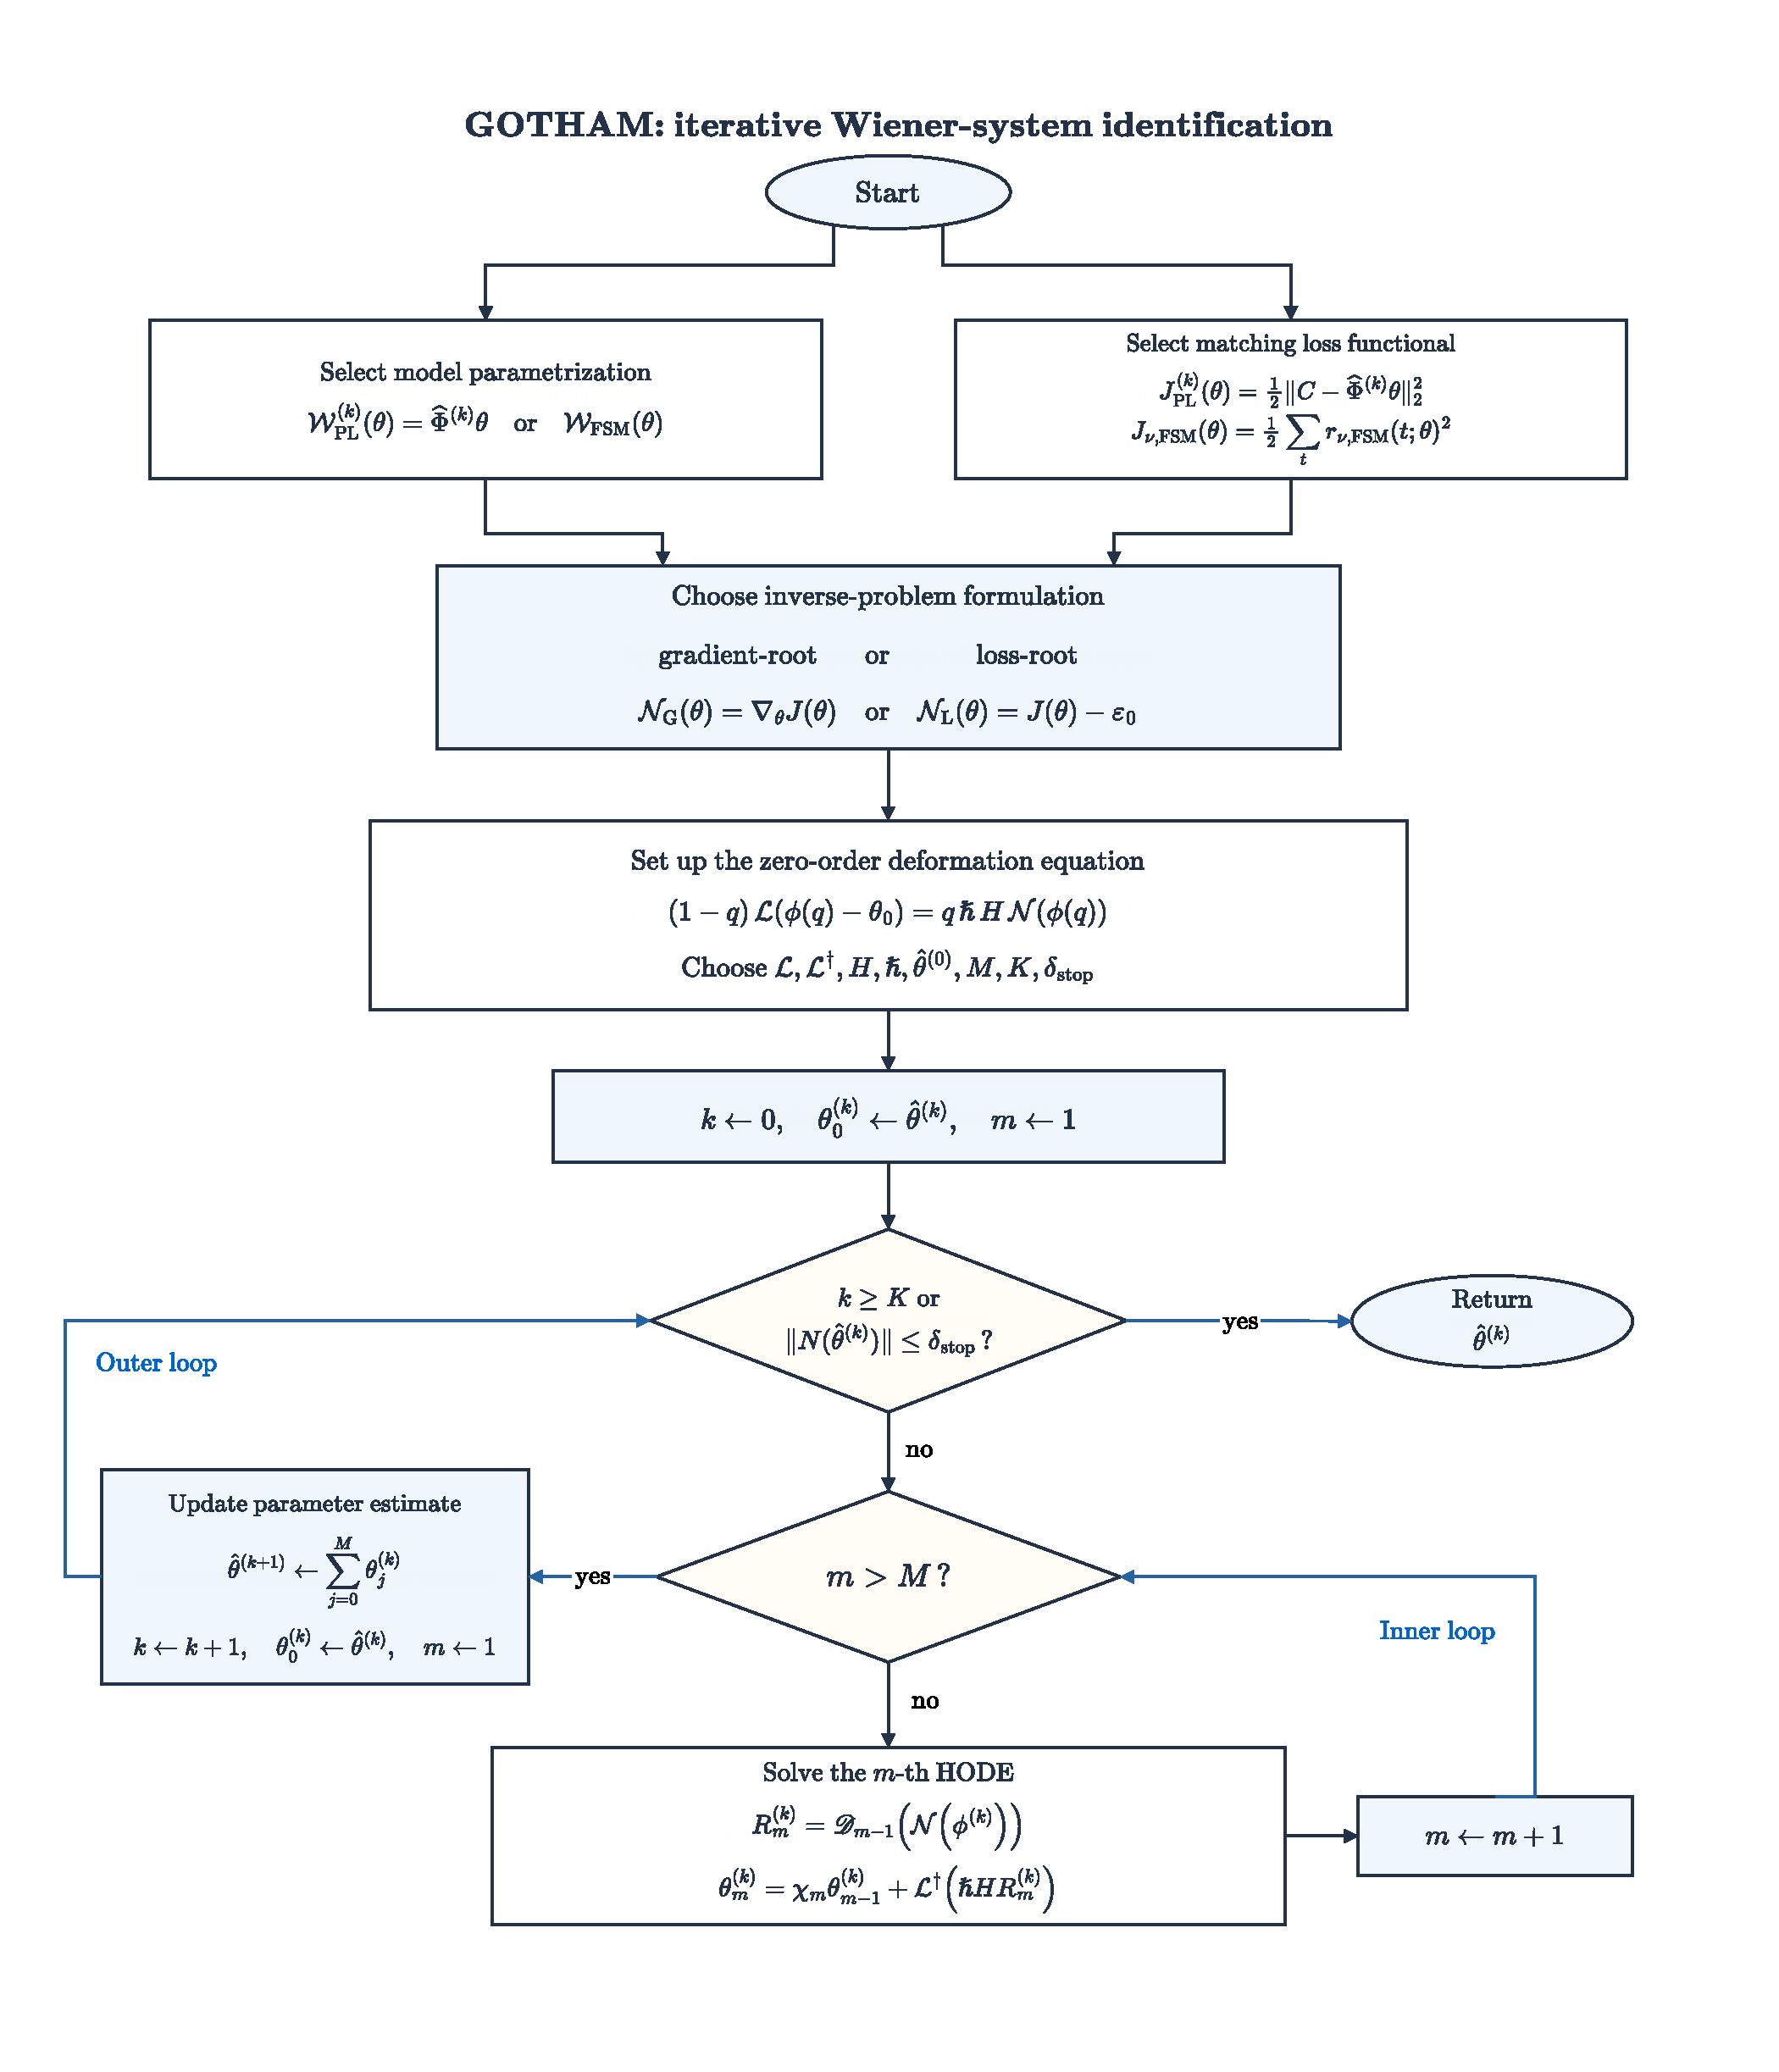
\includegraphics[width=\textwidth,height=.85\textheight,keepaspectratio]
       {figs/GOTHAM_flowchart.pdf}
    \caption{Overall GOTHAM identification procedure for a Wiener system
    with AR output noise. The parametrization and residual operator
    determine the criterion and deformation coefficients.}
    \label{fig:GOTHAM_flowchart}
\end{figure}
}{}
